\documentclass[article,12pt]{elsarticle}
\usepackage[utf8]{inputenc}
\usepackage{graphicx}
\usepackage{booktabs}
\usepackage{subcaption}
\usepackage{amssymb}
\usepackage{flushend}
\usepackage{float}
\usepackage{amsmath}
\usepackage{amsfonts}
\usepackage{dcolumn}
\usepackage{amsthm}
\usepackage{caption}
\usepackage{lmodern}
\usepackage{booktabs}
\usepackage{color}
\usepackage{longtable}
\usepackage{rotating}
\usepackage{etoolbox}
\usepackage{hyperref}
\usepackage{comment}
\usepackage{pdflscape}
\usepackage{comment}
\usepackage[table,xcdraw]{xcolor}
\usepackage[framemethod=TikZ]{mdframed}
\usepackage[a4paper, left=1.5cm, right=1.5cm, top=2cm, bottom=2cm]{geometry}

\begin{document}

\mdfsetup{innertopmargin=10pt,linecolor=blue!20,%
linewidth=2pt,topline=true,
frametitleaboveskip=\dimexpr-\ht\strutbox\relax,}

\begin{frontmatter}
    \title{Laboratorio de Óptica \\ Práctica VII: Polarización}
    \author{López González Andrés$^1$, Reyes Saldivar Ailton Uriel$^2$ y Gante Morales Pedro José$^3$}
    \address{$^1$ Facultad de Ciencias, Universidad Nacional Autónoma de México, México CDMX.}

\begin{abstract}

En esta práctica se exploró la polarización de la luz a través de tres experimentos clave: análisis del grado de polarización de fuentes de luz (láser y LED), medición del ángulo de Brewster en agua y verificación de la Ley de Malus. Se observó que la fuente LED presenta un patrón constante de irradiancia, confirmando su naturaleza no polarizada, mientras que el láser mostró un comportamiento oscilatorio tipo coseno cuadrado, característico de la polarización lineal. El ángulo de Brewster medido fue de \( \theta_B = 0.92^\circ \pm 2.1^\circ \), con un índice de refracción experimental del agua de \( n = 1.30 \pm 0.04 \), en acuerdo con el valor teórico. Finalmente, del ajuste lineal a la Ley de Malus se obtuvo un valor de
 atenuación \( A = 0.53\pm 0.06 \) y una intensidad de fuga \( B = 0.01\pm 0.25 \), confirmando el buen comportamiento del polarizador usado.


\end{abstract}
    
\end{frontmatter}

\section{Introducción}

La \textbf{polarización de la luz} es una manifestación directa de su naturaleza ondulatoria, particularmente de las propiedades del campo eléctrico (\(\vec{E}\)) en una onda electromagnética. De acuerdo con el modelo de ondas planas, el campo eléctrico puede expresarse como:

\begin{mdframed}
\begin{equation}
    \vec{E}(\vec{r}, t) = \vec{E}_0 \, \text{sen}(\vec{k} \cdot \vec{r} - \omega t + \delta),
\end{equation}
\end{mdframed}

donde \(\vec{E}_0\) representa la amplitud del campo eléctrico, \(\vec{k}\) es el vector de onda y \(\delta\) el desfase de fase. Esta forma es solución de la ecuación de onda obtenida a partir de las ecuaciones de Maxwell en ausencia de cargas libres, lo cual valida su comportamiento oscilatorio y transversal en el vacío y en medios dieléctricos homogéneos \cite{griffiths1999, hecht2000}. En este contexto, la \textbf{polarización} se define como la dirección de oscilación del campo eléctrico en el plano perpendicular al vector de propagación \cite{pedrotti2018, Polarizacion}.

Para un análisis más detallado, el campo eléctrico se descompone en componentes ortogonales sobre los ejes \(x\) y \(y\):

\begin{mdframed}
\begin{equation}
    \vec{E}_0 = \begin{pmatrix} E_x \\ E_y \end{pmatrix} = \begin{pmatrix} E_{0x} e^{i\delta_x} \\ E_{0y} e^{i\delta_y} \end{pmatrix},
\end{equation}
\end{mdframed}

donde \(E_{0x}\) y \(E_{0y}\) son las amplitudes respectivas, y \(\delta_x\) y \(\delta_y\) representan sus fases relativas \cite{hecht2000, Polarizacion}.

\subsection{Polarización Lineal}

Cuando la diferencia de fase entre las componentes es un múltiplo entero de \(\pi\), es decir, \(\delta_y - \delta_x = m\pi\), el campo eléctrico oscila en una única dirección, describiendo una línea recta. Este tipo de polarización se denomina \textbf{lineal} y puede orientarse en cualquier ángulo dependiendo de la relación de amplitudes entre \(E_{0x}\) y \(E_{0y}\). Los casos límite incluyen la polarización lineal horizontal (PLH) y vertical (PLV) \cite{pedrotti2018, Polarizacion}.

\subsection{Radiación Dipolar (Modelo Simple)}

El origen microscópico de la luz puede entenderse a través del modelo de \textbf{radiación dipolar}, en el que las cargas oscilantes, generalmente electrones ligados a núcleos atómicos, generan campos eléctricos oscilantes que se propagan como ondas. La intensidad de la radiación observada depende de la dirección respecto a la oscilación del dipolo: es máxima en direcciones perpendiculares y nula en la dirección de oscilación, lo cual explica la polarización inherente de la luz emitida \cite{griffiths1999, Polarizacion}.

\subsection{Luz No Polarizada}

La \textbf{luz natural}, como la emitida por el Sol o fuentes térmicas, es generada por un número enorme de dipolos con orientaciones aleatorias. Esto provoca una superposición de ondas con todas las direcciones de polarización posibles, resultando en una luz sin dirección de polarización preferencial, conocida como \textbf{luz no polarizada} \cite{hecht2000, Polarizacion}.

\subsection{Ley de Malus}

Cuando una onda polarizada linealmente atraviesa un polarizador, la intensidad transmitida \(I\) depende del ángulo \(\theta - \beta\) entre la dirección de polarización de la onda y el eje de transmisión del polarizador. Este fenómeno está descrito por la \textbf{Ley de Malus}:

\begin{mdframed}
\begin{equation}
    I = A(I_0 \cos^2 (\theta - \beta)) + B,
\end{equation}
\end{mdframed}

donde \(I_0\) es la intensidad inicial, \(A\) representa la atenuación del haz que inicide en el  polarizador y \(B\) una componente de fuga, que modela la transmisión residual incluso cuando el eje está cruzado \cite{pedrotti2018, Polarizacion}.

\subsection{Ángulo de Brewster}

Una forma eficiente de generar luz polarizada es mediante la \textbf{reflexión} en una superficie dieléctrica. En particular, cuando la luz incide con un ángulo específico \(\theta_B\), llamado \textbf{ángulo de Brewster}, el rayo reflejado está completamente polarizado perpendicularmente al plano de incidencia. Este ángulo depende de los índices de refracción de los dos medios involucrados y se calcula como:

\begin{mdframed}
\begin{equation}
    \arctan \theta_B = \frac{n_2}{n_1},
\end{equation}
\end{mdframed}

lo que establece una relación geométrica fundamental en óptica para la obtención de luz polarizada por reflexión \cite{griffiths1999, Polarizacion}.

\subsection{Hipótesis}
Si la luz posee un cierto grado de polarización lineal, entonces al hacerla incidir sobre un polarizador y variar su eje de transmisión, se observará una variación periódica en la irradiancia transmitida, que sigue la Ley de Malus. Además, si se observa la luz reflejada en una superficie dieléctrica bajo condiciones específicas, se podrá identificar un ángulo en el cual la luz reflejada esté completamente polarizada, conocido como ángulo de Brewster.

\subsection{Objetivos}
\begin{itemize}
    \item Medir el grado de polarización lineal de diferentes fuentes de luz (láser y LED) analizando la dependencia angular de la irradiancia transmitida a través de un polarizador.
    \item Determinar el ángulo de Brewster para la reflexión en agua mediante observación directa con polarizador y cálculo trigonométrico.
    \item Caracterizar un polarizador mediante el montaje polarizador-analizador, evaluando los parámetros de atenuación (A) e intensidad de fuga (B) a partir del ajuste experimental con la Ley de Malus.
\end{itemize}


\section{Desarrollo Experimental}

\subsection{Grado de Polarización Lineal}
Se utilizó un polarizador lineal hecho de un material dicroico con un eje de transmisión bien definido. Nuestro polarizador está montado sobre una escala angular con una incertidumbre de $\pm 0.5^\circ$. Frente al polarizador, colocamos un radiómetro, el cual cuenta con escalas variables que dependen del rango de irradiancia. Detrás del polarizador, colocamos la fuente de luz (en nuestro caso, un láser y un LED), de la cual queremos conocer el grado de polarización lineal.

Una vez colocado el arreglo, variamos el ángulo del eje del polarizador y registramos la irradiancia correspondiente para cada ángulo, tomando mediciones cada $10^\circ$ desde $0^\circ$ hasta $360^\circ$. Al graficar irradiancia vs. ángulo (datos normalizados), pudimos observar el comportamiento de cada fuente: el LED como una fuente no polarizada y el láser como una fuente linealmente polarizada.

\begin{figure}[H]
    \centering
    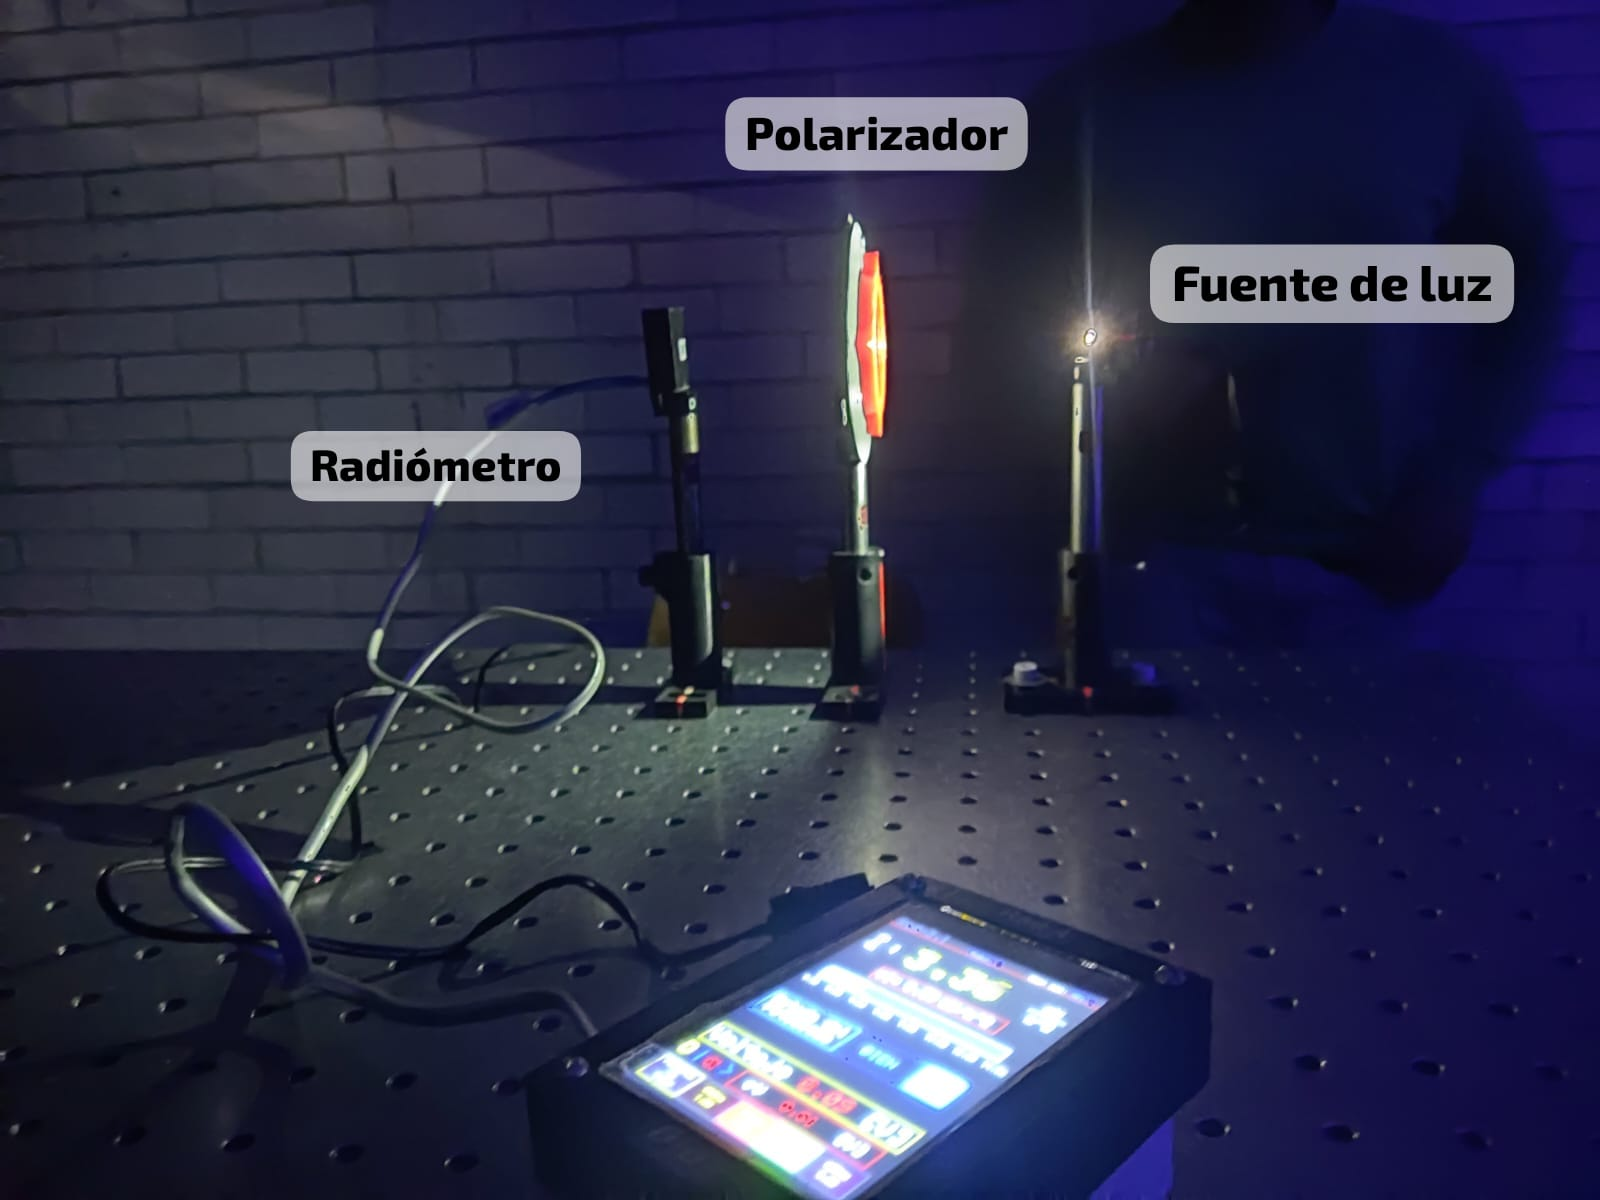
\includegraphics[width=0.5\linewidth]{arreglo 1.jpeg}
    \caption{Arreglo experimental para el grado de polarización lineal.}
    \label{fig:grado_polarizacion}
\end{figure}

\subsection{Ángulo de Brewster}
Sabemos que la ecuación de Brewster relaciona el ángulo de incidencia con los índices de refracción (ver ec. 4 de la introducción). A partir de esta ecuación, podemos calcular el índice de refracción del medio reflejante:

\begin{equation}
    \tan \theta_\beta = n_{\text{agua}}
\end{equation}

Llenamos un recipiente rectangular poco profundo (una sección del fondo era de color negro) y lo colocamos en el piso. Cerca del recipiente, situamos un reflector LED que emite luz no polarizada. El observador tomó un polarizador con su eje de transmisión perpendicular al piso y observó el reflejo de la luz del LED en el agua.

El observador se desplazó hacia adelante y hacia atrás hasta encontrar la mínima intensidad del reflejo, lo que indica que la luz reflejada está polarizada horizontalmente (y, por tanto, no puede atravesar el polarizador, cuyo eje es vertical). Una vez ubicada esta posición, medimos el ángulo de Brewster utilizando un flexómetro: registramos la distancia horizontal ($x$) desde el punto de reflexión hasta los pies del observador y la distancia vertical ($y$) desde el piso hasta los ojos del observador. Finalmente, calculamos el ángulo mediante $\arctan(x/y)$.

Este procedimiento se repitió tres veces, con tres personas diferentes, y se obtuvo un promedio de los resultados.

\begin{figure}[H]
    \centering
    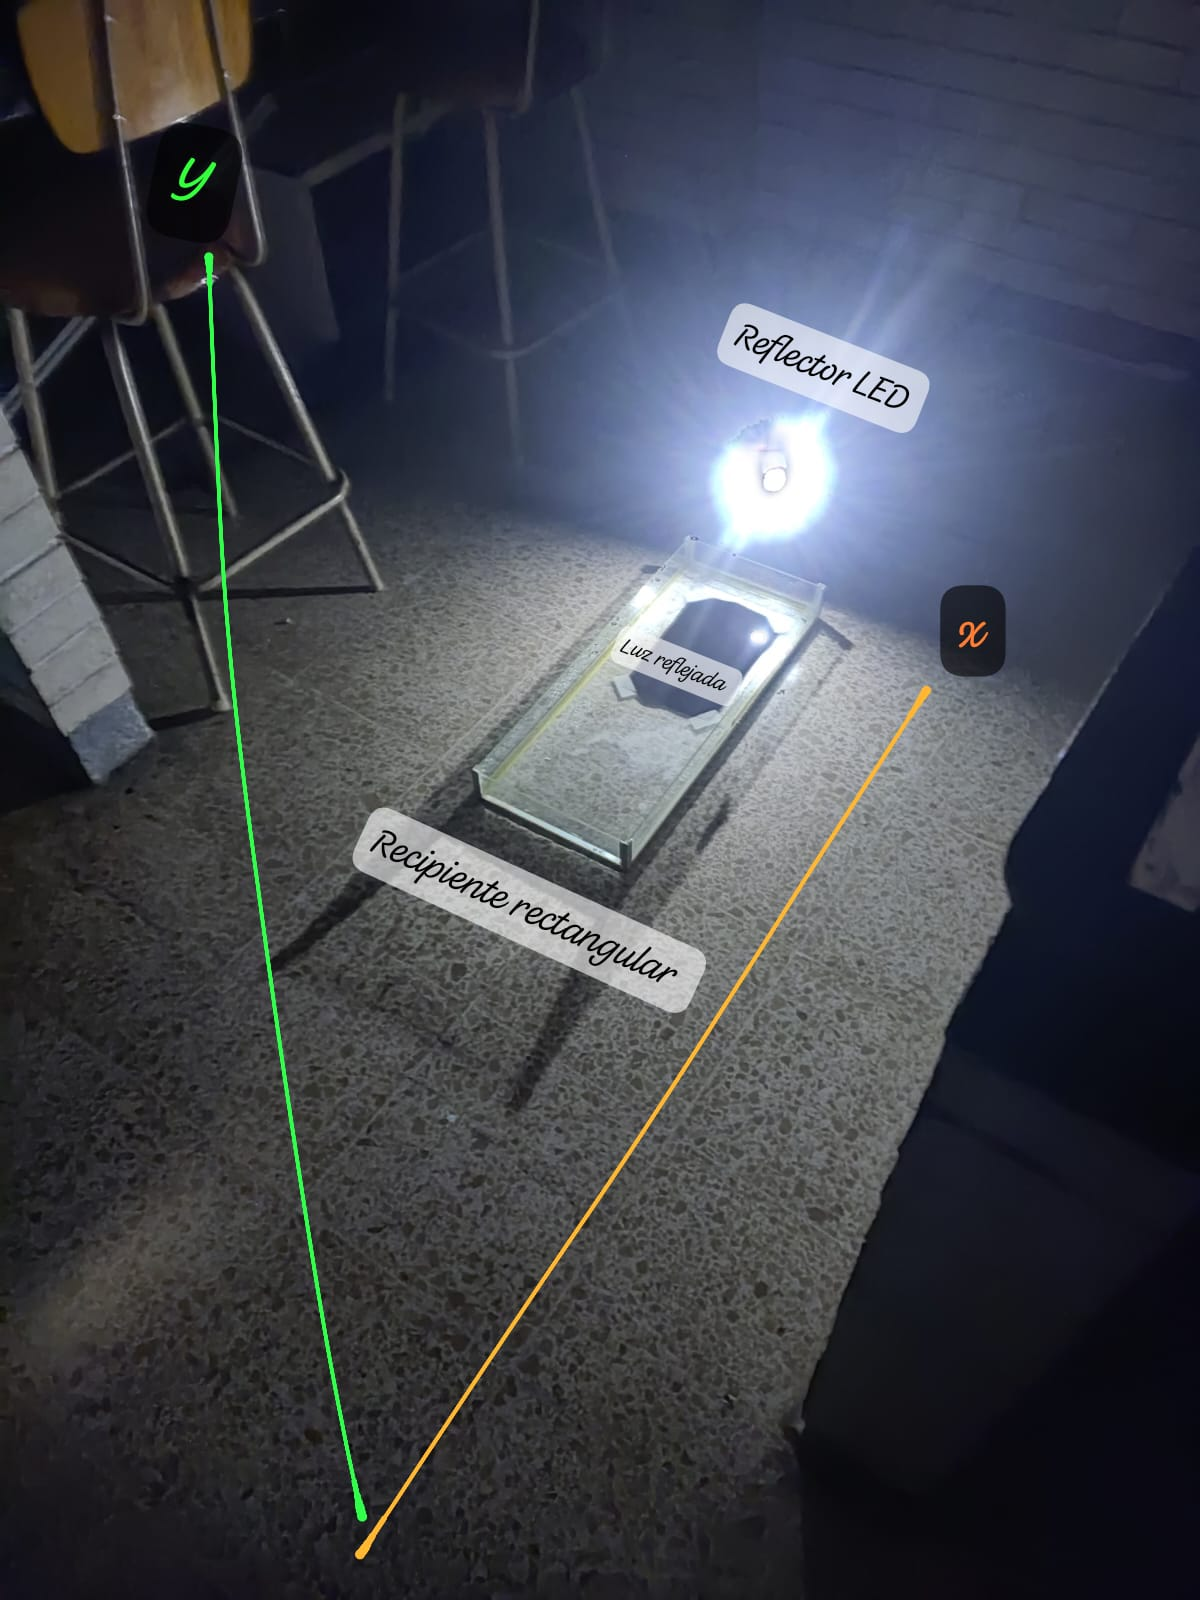
\includegraphics[width=0.3\linewidth]{arreglo 2.png}
    \caption{Arreglo experimental del ángulo de Brewster.}
    \label{fig:brewster}
\end{figure}

\subsection{Ley de Malus}
Para caracterizar un polarizador, utilizamos dos polarizadores, una fuente de luz láser y un radiómetro. El primer polarizador (colocado frente al láser) fija la orientación angular de polarización ($\beta$). El segundo polarizador (analizador) es el que nos interesa caracterizar, y finalmente colocamos el radiómetro para medir la intensidad de la luz transmitida.

Comenzamos con un montaje que solo incluía el primer polarizador, fijando su eje de transmisión en $\beta = 40^\circ$, y medimos la irradiancia inicial ($I_0 = 74.5 \, \text{mW} \pm 1 \, \text{mW}$). Luego, añadimos el analizador entre el primer polarizador y el radiómetro, con su eje de transmisión inicialmente en $0^\circ$. Realizamos un barrido angular de $360^\circ$, tomando mediciones cada $10^\circ$, y registramos la irradiancia junto con su incertidumbre (la cual varió según la escala del radiómetro).

Al graficar irradiancia vs. ángulo ($\theta$), obtuvimos una curva sinusoidal, consistente con la Ley de Malus, donde los máximos coincidieron con $40^\circ$ y $220^\circ$ (como se esperaba teóricamente).

A partir de la ecuación linealizada de la Ley de Malus (ec. 3), calculamos los parámetros $A$ (atenuación) y $B$ (fuga) mediante una gráfica de $I_0 \cos^2(\theta - \beta)$ vs. irradiancia, donde:
\begin{itemize}
    \item La pendiente corresponde a $A$.
    \item La ordenada al origen corresponde a $B$.
\end{itemize}

\begin{figure}[H]
    \centering
    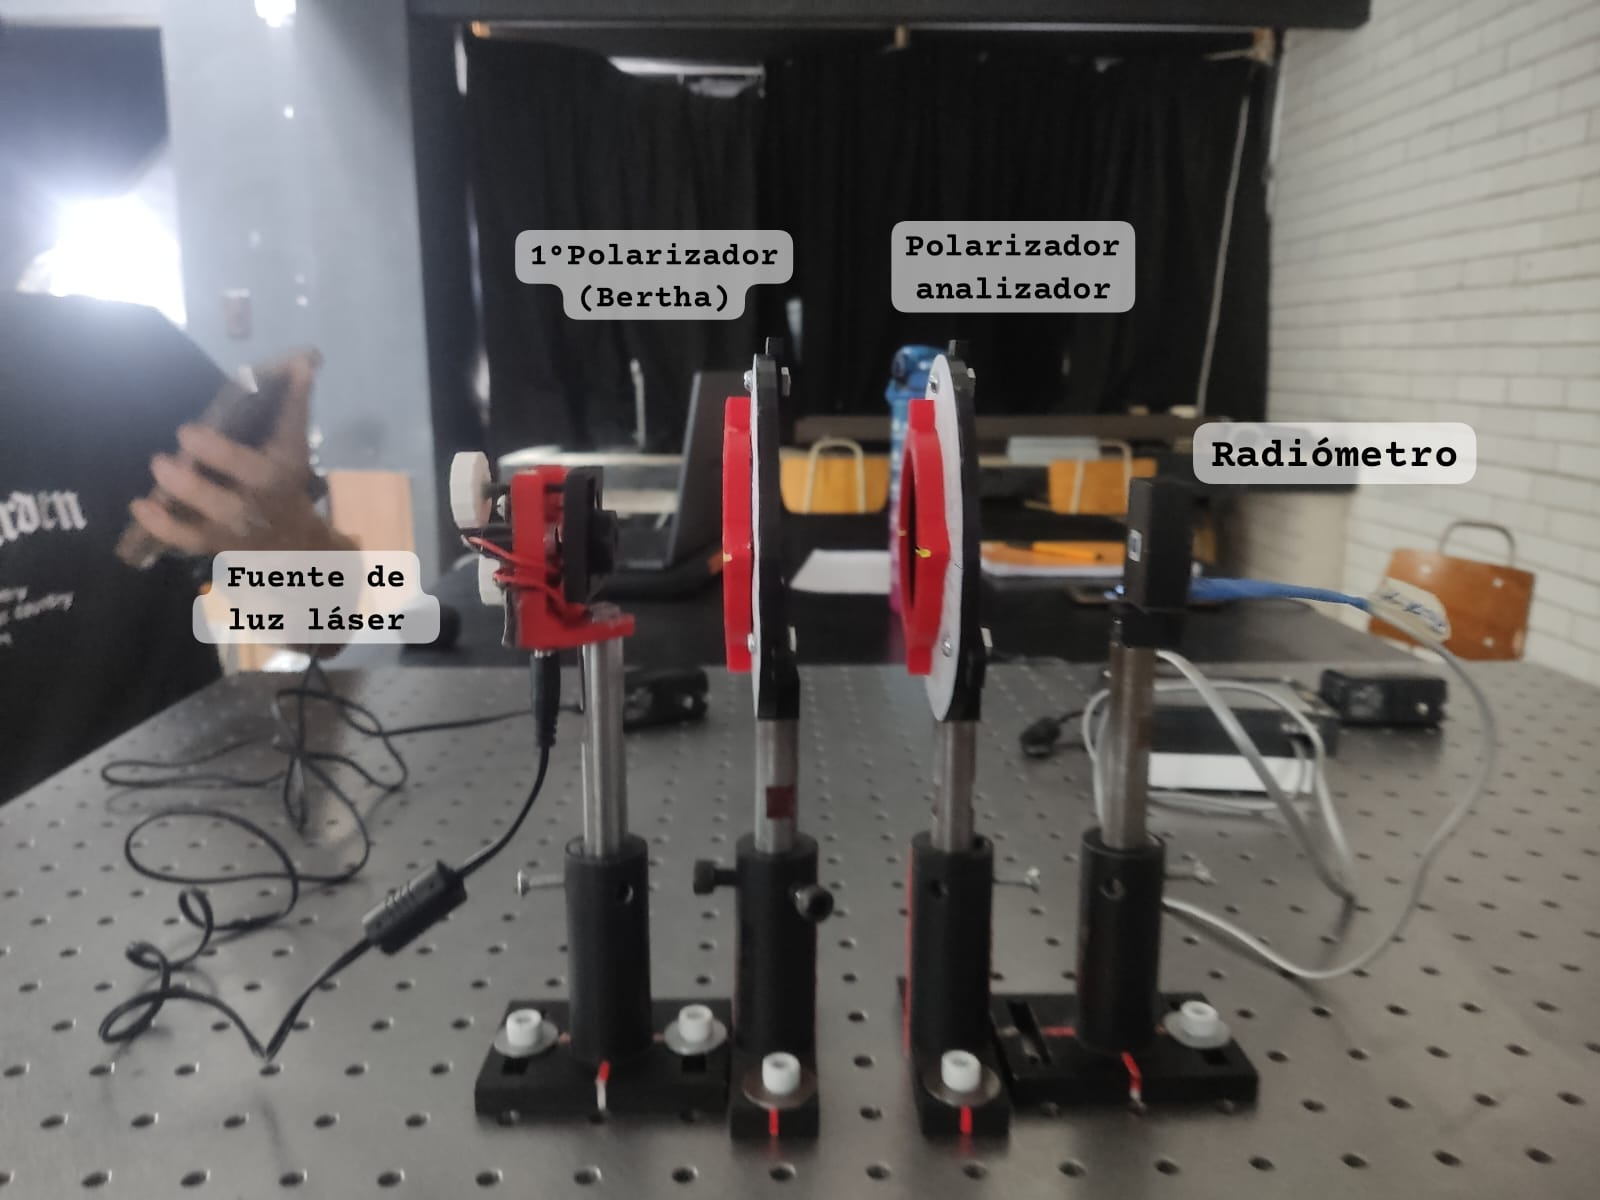
\includegraphics[width=0.5\linewidth]{arreglo 3.jpeg}
    \caption{Arreglo experimental para la Ley de Malus.}
    \label{fig:malus}
\end{figure}

\section{Resultados y tratamiento de datos}

\subsection{Grado de Polarización Lineal}


\begin{table}[H]
\centering
\rowcolors{2}{cyan!15}{white}
\begin{tabular}{|c|c|c|c|c|c|c|}
\hline
\rowcolor{cyan!40}
$\theta$[°] & $\Delta \theta$ [°] & Fondo [mW] & I [mW] & $\Delta$I [mW] & 
 I [Normalizado] & $\Delta I$[Normalizado] \\
\hline
0 & 1 & 0.4 & 1760 & 50 & 0.941 & 0.028\\
10 & 1 & 0.4 & 1590 & 50 & 0.850 & 0.031 \\
20 & 1 & 0.4 & 1340 & 50 & 0.717 & 0.037\\
30 & 1 & 0.4 & 1120 & 10 & 0.599 & 0.009\\
40 & 1 & 0.4 & 760 & 10 & 0.406 & 0.013\\
... & ... & ... & ... & ... & ... & ... \\
320 & 1 & 0.4 & 1390 & 50 & 0.734 & 0.036\\
330 & 1 & 0.4 & 1650 & 50 & 0.882 & 0.030\\
340 & 1 & 0.4 & 1810 & 50 & 0.968 & 0.028\\
350 & 1 & 0.4 & 1870 & 50 & 1 & 0.027\\
360 & 1 & 0.4 & 1810 & 50 & 0.968 & 0.028\\
\hline
\end{tabular}
\caption{Mediciones para grado de polarización lineal para fuente LÁSER}
\end{table}


Para la visualización de la tabla completa en excel la podemos encontrar \cite{Excel}


\begin{table}[H]
\centering
\rowcolors{2}{green!15}{white}
\begin{tabular}{|c|c|c|c|c|c|c|}
\hline
\rowcolor{green!40}
$\theta$[°] & $\Delta \theta$ [°] & Fondo [mW] & I [mW] & $\Delta$I [mW] & 
 I [Normalizado] & $\Delta I$[Normalizado] \\
\hline
0 & 1 & 0.5 & 5.9 & 0.5 & 0.99 & 0.008\\
10 & 1 & 0.5 & 5.98 & 0.5 & 1.0 & 0.08 \\
20 & 1 & 0.5 & 5.75 & 0.5 & 0.96 & 0.09\\
30 & 1 & 0.5 & 5.8 & 0.5 & 0.97 & 0.09\\
40 & 1 & 0.5 & 5.82 & 0.5 & 0.97 & 0.09\\
... & ... & ... & ... & ... & ... & ... \\
320 & 1 & 0.5 & 5.72 & 0.5 & 0.96 & 0.09\\
330 & 1 & 0.5 & 5.66 & 0.5 & 0.95 & 0.09\\
340 & 1 & 0.5 & 5.65 & 0.5 & 0.94 & 0.09\\
350 & 1 & 0.5 & 5.65 & 0.5 & 0.94 & 0.09\\
360 & 1 & 0.5 & 5.66 & 0.5 & 0.95 & 0.09\\
\hline
\end{tabular}
\caption{Mediciones para grado de polarización lineal para fuente LED}
\end{table}



Para la visualización de la tabla completa en excel la podemos encontrar \cite{Excel}

\begin{figure}[H]
    \centering
    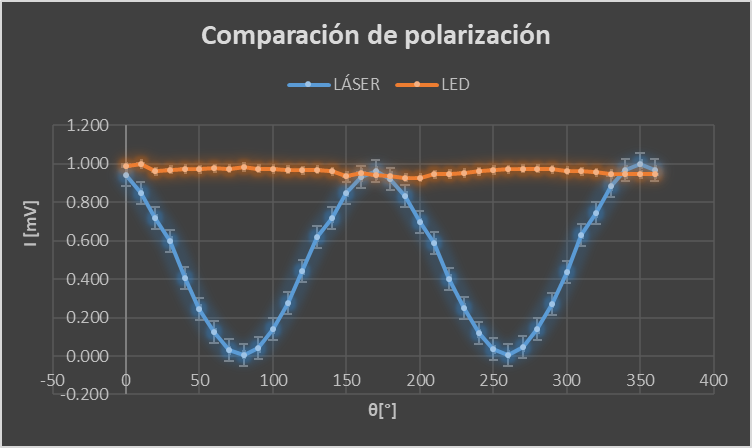
\includegraphics[width=0.75\linewidth]{Grado de polarización Lineal.png}
    \caption{Gráfica de polarización de 2 diferentes fuentes}
    \label{grafica 1}
\end{figure}

Podemos observar en la gráfica \ref{grafica 1} que dado la irradiacian de la fuente LED no cambia considerablemente respecto al eje del polarizador, se puede concluir que se trata de una fuente de luz NO polarizada. No obstante para el caso del LÁSER es posible observar un comportamiento tipo de coseno cuadrado, como el que se predice en la ley de malus para fuentes con polarización lineal, cabe agregar que la función cuenta con desfase respecto al origen de $0°$, donde las máximas irradiancias están en 0°, 180° y 360° aproximadamente.


\subsection{Ángulo de Brewster}

\begin{table}[H]
\centering
\rowcolors{2}{orange!15}{white}
\begin{tabular}{|c|c|c|c|c|c|c|c|c|}
\hline
\rowcolor{orange!40}
$D_{\text{Obs}}$ [cm] & $\Delta D$ [cm] & $h_{\text{Obs}}$ [cm] & $\Delta h$ [cm] & $\theta_B$ Obs [°] & $\Delta \theta_B$ Obs [°] & $n_{\text{agua}}$ & $\Delta n_{\text{agua}}$ & $n_{\text{teo}}$ \\
\hline
1.977 & 1 & 1.52 & 1 & 0.92 & 2.1 & 1.30 & 0.04 & 1.33 \\
\hline
\end{tabular}
\caption{Mediciones y resultados del ángulo de Brewster}
\label{Brewster}
\end{table}

Con los datos medidos que encontramos en la tabla \ref{Brewster}, podemos calcular el índice de refracción del agua (medio reflejante) $n_{agua}=1.30\pm0.04$ (incertidumbre calculada con la ecuacióm 6 en el Anexo) que coincide con el teórico de $n_{teórico}=1.33$

\subsection{Ley de Malus}

\begin{table}[H]
\centering
\rowcolors{2}{purple!15}{white}
\begin{tabular}{|c|c|c|c|}
\hline
\rowcolor{purple!40}
$\beta$[°] & $\Delta \beta$ [°] & $I_0$ [mW] & $\Delta I_0$ [mW] \\
\hline
40 & 1 & 74.5 & 1 \\
\hline
\end{tabular}
\caption{Mediciones para la Ley de Malus}
\end{table}



\begin{table}[H]
\centering
\rowcolors{2}{blue!20}{white}
\begin{tabular}{|c|c|c|c|c|c|}
\hline
\rowcolor{blue!40}
$\theta$[°] & $\Delta \theta$ [°] & I [mW] & $\Delta$I [mW] & $I_0[\cos(\theta - \beta)]^2$ & $\Delta [I_0[\cos(\theta - \beta)]^2]$ \\
\hline
0 & 1 & 22.4 & 1 & 44 & 15 \\
10 & 1 & 29.9 & 1 & 56 & 5 \\
20 & 1 & 35.1 & 1 & 66 & 11 \\
30 & 1 & 39.2 & 1 & 72 & 14 \\
40 & 1 & 41.4 & 1 & 75 & 16 \\
50 & 1 & 41.1 & 1 & 72 & 14 \\
... & ... & ... & ... & ... & ... \\
310 & 1 & 0.5 & 0.5 & 0 & 1 \\
320 & 1 & 0.68 & 0.5 & 2 &  1\\
330 & 1 & 2.81 & 0.5 & 9 & 3 \\
340 & 1 & 7.46 & 0.5 & 19 & 4 \\
350 & 1 & 13.27 & 0.5 & 31 & 13 \\
360 & 1 & 19.1 & 1 & 44 & 12 \\
\hline
\end{tabular}
\caption{Mediciones para la Ley de Malus (Láser)}
\end{table}


Para la visualización de la tabla completa en excel la podemos encontrar \cite{Excel}

\begin{figure}[H]
    \centering
    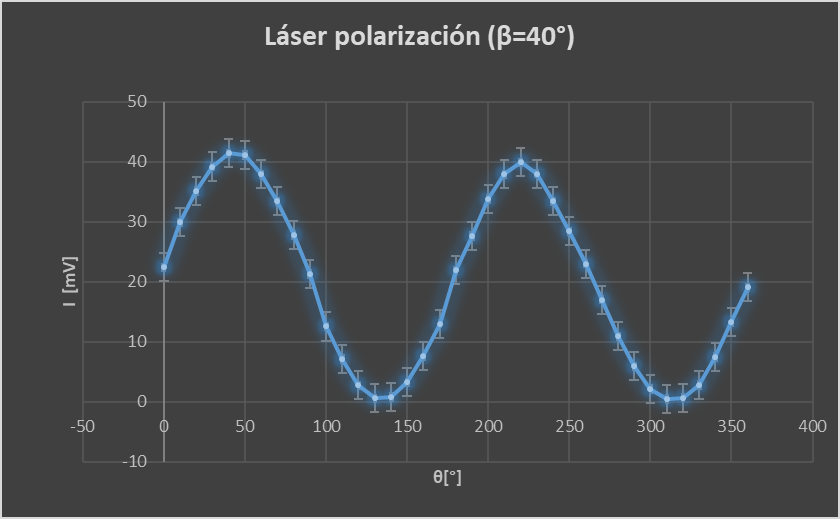
\includegraphics[width=0.75\linewidth]{Ley de Malus 1.png}
    \caption{Gráfica de $\theta$ [°] vs Irradiancia [mV]}
    \label{Ley de Malus 1}
\end{figure}

En la gráfica \ref{Ley de Malus 1} podemos observar un comportamiento sinusoidal acorde con la ley de malus, con máximos en 40° y 220° aproximadamente, con lo se confirma que el ángulo $\beta$ corresponde a 40° grados.

Por otro lado para calcular los coeficientes A y B usamos la forma linealizada de la ley de Malus (Ec. 3) , el valor de A debe tener un valor entre 0 y 1 debido a otros tipos de absorción del material, mientra que B debe tener un valor muy bajo respecto a la intensidad máxima de la fuente de entrada. Con esta linealización construímos otra gráfica con las variables $I_0cos^2(\theta - \beta)$ contra la Irradiancia. De esta relación podemos extraer la relación de identidad entre la pendiente m con el factor A y de B con la ordenada al origen (Usando las ecuaciones 8 y 9 del anexo, calculamos la incertidumbre nominal para los coefiencientes A y B). 

\begin{figure}[H]
    \centering
    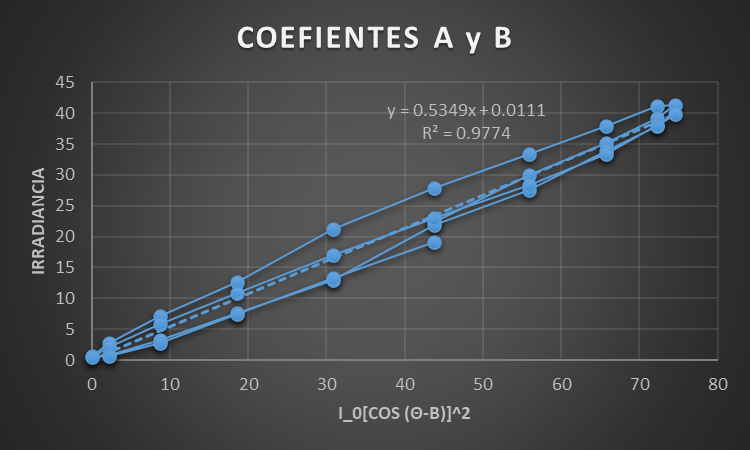
\includegraphics[width=0.75\linewidth]{Ley de Malus 2.png}
    \caption{Grafica para calcular los coefiecientes A y B}
    \label{fig:enter-label}
\end{figure}

\begin{table}[H]
\centering
\rowcolors{2}{green!15}{white}
\begin{tabular}{|c|c|c|c|}
\hline
\rowcolor{purple!40}
A & $\Delta A$ & B & $\Delta B$  \\
\hline
0.53 & 0.06 & 0.01 & 0.25\\
\hline
\end{tabular}
\caption{Mediciones para la Ley de Malus}
\end{table}


\section{Conclusiones}

\begin{enumerate}
    \item El experimento demostró que la polarización lineal de la luz láser puede verificarse empíricamente mediante la variación de la irradiancia con el ángulo del polarizador, siguiendo una dependencia de tipo \( \cos^2(\theta - \beta) \), como predice la Ley de Malus.
    
    \item La fuente LED presentó una irradiancia prácticamente constante respecto al ángulo del polarizador, confirmando su naturaleza como luz no polarizada.
    
    \item La medición del ángulo de Brewster permitió estimar un índice de refracción del agua de \( n = 1.30 \pm 0.40 \), valor coherente con el teórico (\( n_{\text{teo}} = 1.33 \)), validando el método óptico usado.
    
    \item La linealización de la Ley de Malus permitió caracterizar el polarizador usado, arrojando un coeficiente de atenuación \( A = 0.53 \) y una fuga \( B = 0.01 \), lo cual indica un buen nivel de polarización y baja transmisión residual.
    
    \item La práctica permitió reforzar el entendimiento del comportamiento de la luz como onda electromagnética transversal, así como de los mecanismos físicos detrás de la polarización por transmisión y reflexión.
\end{enumerate}

\begin{thebibliography}{9}

\bibitem{griffiths1999}
D. J. Griffiths, \textit{Introduction to Electrodynamics}, 3ª edición, Prentice Hall, 1999.

\bibitem{hecht2000}
E. Hecht, \textit{Óptica}, 3ª edición, Addison Wesley, 2000.

\bibitem{pedrotti2018}
F. L. Pedrotti, L. M. Pedrotti, L. S. Pedrotti, \textit{Introduction to Optics}, 3ª edición, Cambridge University Press, 2018.

\bibitem{Polarizacion}
Erick Barrios Barocio; Roxette Ramírez Arvidez, \textit{Polarización}, Óptica v.2025. \href{https://tsikbal.github.io/P%C3%A1ginas/%C3%81reas/F%C3%ADsica/%C3%93ptica/Optica_Fisica/Polarizaci%C3%B3n.html}{Enlace al documento}

\bibitem{Excel} A. Reyes, S. Tabla de Polarización, Archivo Excel. 2024. Disponible en: \href{https://docs.google.com/spreadsheets/d/1_yYCZ7q34UFFrDisqF6pmfBwCw3KAzEm/edit?usp=sharing&ouid=112625838925660900694&rtpof=true&sd=true}{Enlace al documento}
\end{thebibliography}


\section*{Anexo}

\begin{mdframed}
\begin{equation}
\Delta n_2 = 
= \sqrt{
    \left( \frac{h}{D^2 + h^2} \Delta D \right)^2 
    + \left( \frac{D}{h^2 + D^2} \Delta h \right)^2}
\end{equation}
\end{mdframed}

\begin{mdframed}
\begin{equation}
\Delta \theta_B = \frac{\partial}{\partial n_2} \left( \arctan(n_2) \right) \Delta n_2 = \frac{\Delta n_2}{1 + n_2^2}
\end{equation}
\end{mdframed}

\begin{mdframed}
\begin{equation}
\Delta A = \sqrt{
    \left( \frac{\Delta I}{I_0 \cos^2(\theta - \beta)} \right)^2 
    + \left( \frac{2(I - B) \sin(\theta - \beta)}{I_0 \cos^3(\theta - \beta)} \Delta \theta \right)^2
}
\end{equation}
\end{mdframed}

\begin{mdframed}
\begin{equation}
\Delta B = \sqrt{
    \left( \Delta I \right)^2 
    + \left( 2 A I_0 \cos(\theta - \beta) \sin(\theta - \beta) \Delta \theta \right)^2
}
\end{equation}
\end{mdframed}

\end{document}